\documentclass[11pt]{article}
\usepackage{classTools}

\drafttrue

\begin{document}

% To include a problems set header, use the psHeader command
\psHeader{4}{Wed Oct. 12, 2022 (11:59pm)}

\textbf{Your name: }

\textbf{Collaborators: }

\textbf{No. of late days used on previous psets: }

\textbf{No. of late days used after including this pset: }

\begin{enumerate}
    \item (Randomized Algorithms in Practice)  
    \begin{enumerate}
        \item Implement Randomized QuickSelect, filling in the template we have given you in the \href{https://github.com/Harvard-CS-120/cs120/tree/main/fall2022/psets}{Github repository}.  
        
        \item 
        In the repository, we have given you datasets $x_n$ of key-value pairs of varying sizes to experiment with.  For each dataset $x_n$ and any given number $k$, you will compare two ways of answering the $k$ selection queries
        Select$(x_n,[n/k])$, Select$(x_n,[2n/k]), \ldots$, Select$(x_n,[(k-1)n/k])$ on $x_n$, where $[\cdot]$ denotes rounding to the nearest integer:
        \begin{enumerate}
            \item Running Randomized QuickSelect $k$ times
            \item Running MergeSort (provided in the repository) once and using the sorted array to answer the $k$ queries
        \end{enumerate}
        Specifically, you will compare the {\em distribution} of runtimes of the two approaches for a given pair $(n,k)$ by running each approach many times and creating density plots of the runtimes.  The runtimes will vary because Randomized QuickSelect  is randomized, and because of variance in the execution environment (e.g. what other processes are running on your computer during each execution).
        
        We have provided you with the code for plotting. Before plotting, you will need to implement MergeSortSelect, which extends MergeSort to answer $k$ queries. Your goal is to use these experiments and the resulting density plots to propose a value for $k$, denoted $k^*_n$, at which you should switch over from Randomized QuickSelect to MergeSort for each given value of $n$. Do this by experimenting with the parameters for $k$ (code is included to generate the appropriate queries once the $k$s are provided) and generate a plot for each experiment.  Explain the rationale behind your choices, and submit a few density plots for each value of $n$ to support your reasoning.  (There is not one right answer, and it may depend on your particular implementation of QuickSelect.) 

        \item Extrapolate to come up with a simple functional form for $k^*_n$, e.g. something like $k^*(n)=3\sqrt{n}+6$ or $k^*(n)=10\log n$. (Again there is not one right answer.)

        \item (*optional)  One way to improve Randomized QuickSelect is to choose a pivot more carefully than by picking a uniformly random element from the array. A possible approach is to use the \textit{\textbf{median-of-3}} method: choose the pivot as the median of a set of 3 elements randomly selected from the array. Add Median-of-3 QuickSelect to the experimental comparisons you performed above and interpret the results.
    \end{enumerate}


    \item (Dictionaries and Hash Tables) 
    Recall the DuplicateSearch problem from Lecture 3. Show that DuplicateSearch can be solved by a Las Vegas algorithm with expected runtime $O(n)$ using a dictionary data structure.  (You can quote the runtimes of the implementation of a dictionary data structure from Lecture 9 without proof.) 

    \item  (Rotating Walks)  
    Suppose we are given $k$ digraphs on the same vertex set, $G_0=(V,E_0), G_1=(V,E_1), \ldots, G_{k-1}=(V,E_{k-1})$.  For vertices $s,t\in V$, a {\em rotating walk} with respect to $G_0,\ldots,G_{k-1}$ from $s$ to $t$ is a sequence of vertices $v_0,v_1,\ldots,v_{\ell}$ such that $v_0=s$, $v_\ell=t$, and $(v_i,v_{i+1})\in E_{i \bmod k}$ for $i=0,\ldots,\ell-1$.  That is, we are looking for walks that rotate between the digraphs $G_0,G_1,\ldots,G_{k-1}$ in the edges used.
    \begin{enumerate}
        \item Show that the problem of finding a Shortest Rotating Walk from $s$ to $t$ with respect to $G_0,\ldots,G_{k-1}$ 
        can be reduced to Single-Source Shortest Walks via a reduction that makes one oracle call on 
        a digraph $G'$ with $kn$ vertices and $m_0+m_1+\cdots+m_{k-1}$ edges, where $n=|V|$ and $m_i=|E_i|$.
        We encourage you to index the vertices of $G'$ by pairs $(v,j)$ where $v\in V$ and $j\in [k]$. 
        Analyze the running time of your reduction and deduce that the Shortest Rotating Walk can be found in time $O(kn+m_0+\cdots+m_{k-1})$.
        \label{part:ReduceToOrdinary}  To test your reduction and algorithm, try running through the example in Part~\ref{part:BFS}.
        
        \item \label{part:BFS} Run your algorithm from Part~\ref{part:ReduceToOrdinary} on the following pair of graphs $G_0$ and $G_1$ to find the Shortest Rotating Walk from $s=(a,0)$ to $t=(c,0)$; this will involve solving Single-Source Shortest Walks on a digraph $G'$ with $2\cdot 8=16$ vertices. Fill out the table provided below with the BFS frontier in $G'$ at each iteration, labelling the vertices of $G'$ as $(a, 0),(b, 0),\ldots,(g,0),(a,1),(b,1),\ldots,(g,1)$, and for each vertex $v$ in the table, drawing an arrow in the table from $v$'s BFS predecessor to $v$. 
%        \salil{is this the same example as from last year?  May be good to change it.} \salil{where's the table?}

            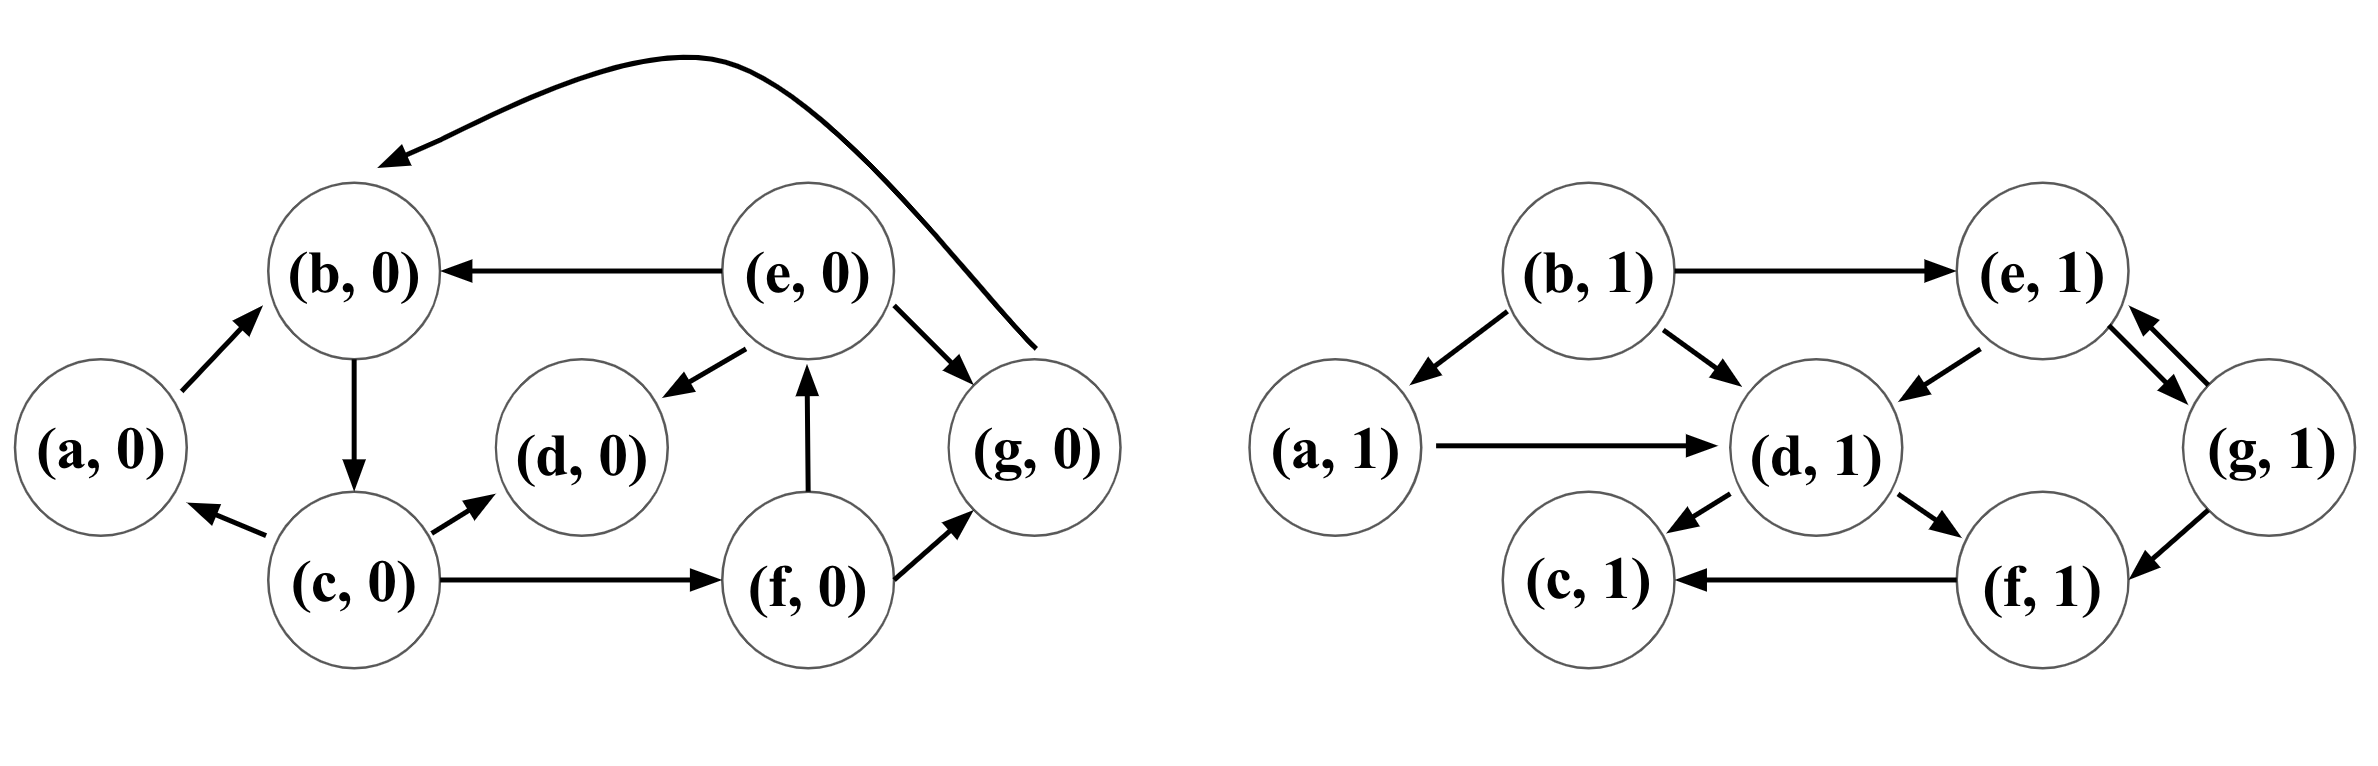
\includegraphics[width=14cm]{ps4_graphs_new.png}

        \begin{table}[ht]
        \centering
        \begin{tabular}{c|c|c}
            $d$ & Frontier $F_d$& Predecessor Relationships \\
            \hline
              & & \\
              & & \\
              & & \\
              & & \\
        \end{tabular}
    \end{table}
    \item 
        A group of three friends decides to play a new cooperative game (similar to the real-life board game Magic Maze).  They rotate turns moving a shared single piece on an $n\times n$ grid.  The piece starts in the lower-left corner, and their goal is to get the piece to the upper-right corner in as few turns as possible.  Many of the spaces on the grid have visible bombs, so they cannot move their piece to those spaces.  Each player is restricted in how they can move the piece.  Player 0 can move it like a chess-rook (any number of spaces vertically or horizontally, provided it does not cross any bomb spaces). Player 2 can move it like a chess bishop (any number of spaces diagonally in any direction, provided it does not cross any bomb spaces).  Player 3 can move it like a chess knight (move to any non-bomb space that is two steps away in a horizontal direction and one step away in a vertical direction or vice-versa).   Using Part~\ref{part:BFS}, show that given the $n\times n$ game board (i.e., the locations of all the bomb spaces), they can find the quickest solution in time $O(n^3)$.  
        (Hint: give a reduction, mapping the given grid to an appropriate instance $(G_0,G_1,\ldots,G_{k-1},s,t)$ of Shortest $k$-Rotating Paths.)
    \end{enumerate}
\end{enumerate}
\end{document}